
%(BEGIN_QUESTION)
% Copyright 2014, Tony R. Kuphaldt, released under the Creative Commons Attribution License (v 1.0)
% This means you may do almost anything with this work of mine, so long as you give me proper credit

Calculate the necessary value for resistor $R_2$ in order for it to dissipate 0.85 watts of power, as well as the voltage output by the current source with that value of $R_2$ in the circuit:

$$\includegraphics[width=15.5cm]{i03045x01.eps}$$

$R_2$ = 

\vskip 10pt

$V_{supply}$ = 

\vskip 10pt

\underbar{file i03045}
%(END_QUESTION)





%(BEGIN_ANSWER)

$R_2$ = 531.25 $\Omega$

\vskip 10pt

$V_{supply}$ = 61.25 volts


%(END_ANSWER)





%(BEGIN_NOTES)

{\bf This question is intended for exams only and not worksheets!}.

%(END_NOTES)

